\documentclass[10pt,a4paper,oneside,fleqn]{report}
\usepackage{geometry}
\geometry{a4paper,left=20mm,right=20mm,top=1cm,bottom=2cm}
\usepackage[utf8]{inputenc}
%\usepackage{ngerman}
\usepackage{amsmath}                % brauche ich um dir Formel zu umrahmen.
\usepackage{amsfonts}                % brauche ich für die Mengensymbole
\usepackage{graphicx}
\setlength{\parindent}{0px}
\setlength{\mathindent}{10mm}
\usepackage{bbold}                    %brauche ich für die doppel Zahlen Darstellung (Einheitsmatrix z.B)
\usepackage[linktocpage={false}]{hyperref}


\usepackage{color}
\usepackage{titlesec} %sudo apt-get install texlive-latex-extra

\definecolor{darkblue}{rgb}{0.1,0.1,0.55}
\definecolor{darkred}{rgb}{0.55,0.2,0.2}

\titleformat{\chapter}[display]{\color{darkred}\normalfont\huge\bfseries}{\chaptertitlename\
\thechapter}{20pt}{\Huge}

\titleformat{\section}{\color{darkblue}\normalfont\Large\bfseries}{\thesection}{1em}{}
\titleformat{\subsection}{\color{darkblue}\normalfont\Large\bfseries}{\thesection}{1em}{}

% Notiz Box
\usepackage{fancybox}
\newcommand{\notiz}[1]{\vspace{5mm}\ovalbox{\begin{minipage}{1\textwidth}#1\end{minipage}}\vspace{5mm}}

\usepackage{cancel}



%\includegraphics[width=0.75\textwidth]{thepic.png}
%couchdb db=physik
%couchdb id=festkvorles05_Elastische_Eigenschaften
%couchdb tags=festk
%couchdb pdflink=http://wernwa-physik-ka.googlecode.com/svn/festk/kap05.pdf

\begin{document}
\tableofcontents
\setcounter{chapter}{4}
\chapter{Eleastische Eigenschaften}


\(\vec r \) nach Deformation \(\rightarrow \vec r + \vec U(\vec r)\) mit \(\vec U\)-Verformung.
Die Freie Energie:

\[ \mathcal F = \int_V d\vec r \frac 1 2 \sum_{\alpha
  \beta\gamma\delta}\underbrace{E_{\alpha
    \beta\gamma\delta}}_{\text{Tensor}}\frac{\partial U_\alpha(\vec
  r)}{dr_\beta}\cdot
\frac{\partial U_\gamma(\vec r)}{dr_\gamma} \]

\(E_{\alpha\beta\gamma\delta}\rightarrow 81= 3^4 \) Komponenten:
Symmetrie mit 45 unabhängigen Komponenten \(\alpha\beta \leftrightarrow
\gamma\delta\) ändert sich nicht unter Drehung von \underline{nicht}
deformierte Festk.

\(E_{\alpha\beta\gamma\delta}-E_{\beta\alpha\gamma\delta}+E_{\alpha\beta\delta\gamma}+E_{\beta\alpha\delta\gamma}=0\);nur 21 Komponenten.

Dehnungstensor (strain tensor): 

\[e_{\alpha\beta}= e^{\leftrightarrow} = [e] = \frac 1 2 [\frac {\partial U_\alpha(\vec
  r)}{dr_\beta}\cdot \frac{\partial U_\gamma(\vec r)}{dr_\gamma}] 
\]

Spannungstensor: 

\[ \sigma_{\alpha\beta} = \sigma^\leftrightarrow = [\sigma] =
\sum_{\alpha\beta}
\underbrace{C_{\alpha\beta\gamma\delta}}_{elastizitaetstensor}e_{\gamma\delta} \]

\[ \mathcal F = \sum_{\alpha\beta}\int \vec r \frac 1 2
e_{\gamma\delta} \sigma_{\gamma\delta}\]

\[ C_{\alpha\beta\gamma\delta} = \frac 1
4(E_{\alpha\beta\gamma\delta}+E_{\beta\alpha\gamma\delta}+E_{\alpha\beta\delta\gamma}+E_{\beta\alpha\delta\gamma}) 
\]

Arbeit = Länge * Kraft

\section{Elastische Konstanten für kubische Kristalle}

\[ C_{\alpha\alpha\alpha\alpha} \stackrel{\mathrm{def}}= C_{11} \]
\[ C_{\alpha\alpha\beta\beta} \stackrel{\mathrm{def}}= C_{12} \]
\[ C_{\alpha\beta\alpha\beta} \stackrel{\mathrm{def}}= C_{44} \]

für isotropen Materialien \(C_{11}-C_{12}=2C_{44}\) nur 2 unabhänige
Komponenten

Lamé-Konstanten \(\lambda \stackrel{\mathrm{def}}= C_{12}\);  \(\mu
\stackrel{\mathrm{def}}= C_{44}\)

\[ \mathcal F = \frac 1 2 C_{11} (e^2_{xx}+e^2_{yy}+e^2_{zz})+
\frac 1 2 C_{44} (e^2_{yz}+e^2_{zx}+e^2_{xy})+
C_{12} (e^2_{yy}e^2_{zz}+e^2_{zz}e^2_{xx}+e^2_{xx}e^2_{yy})
\]

Volumen-Kompression: \(e^2_{xx}=e^2_{yy}=e^2_{zz}=\frac 1 3 \delta\);
\(\mathcal F = \frac 1 6(C_{11}+C_{12})\delta^2\);

Kompressionsmodul: \(B\frac{C_{11}+2C_{12}}{3} =
\frac{3\lambda+2\mu}{3}\), \(\mathcal F = \frac 1 2 B\delta^2\)

Kompressibilität: \(\kappa = \frac 1 B = - \frac 1 V \cdot
\frac{dV}{dp}\)

Elastizitätsmodul (Youngscher Modul) \(E =
\frac{\text{Spannung}}{\text{Dehnung}} \approx \frac{d \sigma}{de} =
\frac{\mu(3\lambda + 2\mu}{\lambda +\mu}\)

\section{Konstanten für kubische Kristalle}

Elastizitätskraft: \(f_\alpha(\vec r) = \rho \ddot u_\alpha
(\vec r) = \sum_\beta \frac {\partial \sigma_{\alpha\beta}(\vec r)}{dr_\beta}\)

\section{Schallwellen}

\begin{itemize}
\item longitudinale 
\(\vec q\) Wellenvektor. \(\vec q || \vec u\)
\item transversale \(\vec q \bot  \vec u\)
\end{itemize}


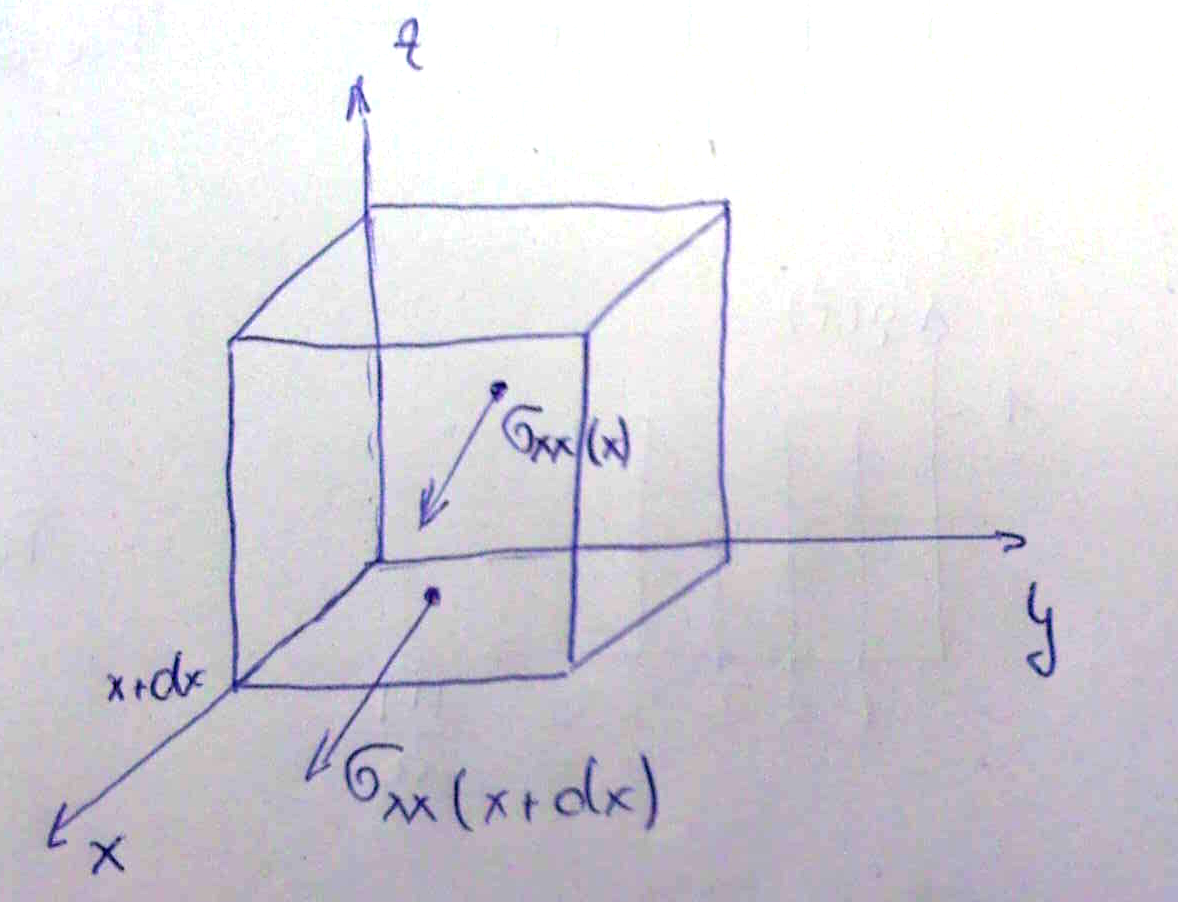
\includegraphics[width=0.75\textwidth]{kap05_01.png}

\[ df_x = \sigma_{xx}(x+dx) - \sigma_{xx}(x)dxdz =
\frac{\partial\sigma_{xx}}{\partial x}dxdydz \]

\[ \rho \frac{\partial^2 U_x}{\partial t^2} =
\frac{\partial\sigma_{xx}}{\partial x} \]

\[ \sigma_{xx} = O_{11}e_{xx} = C_{11}\frac{\partial U_x}{\partial x} \]
\[ \Rightarrow  \rho \frac{\partial^2 U_x}{\partial t^2} = C_{11}\frac{\partial^2 U_x}{\partial x^2}\]

allgemeine Form  

\[\rho \frac{\partial^2 U_x}{\partial t^2} =  \sum_{\beta\gamma\delta} C_{\alpha\beta\gamma\delta}\frac{\partial U_\delta}{\partial r_\beta\partial_\gamma} \]

Lösung:

\[ U_\alpha = U_{o\alpha}exp(-i\omega t + i \vec q\cdot \vec r )\]

f kubische Kristalle

\[\rho \frac{\partial^2 U_x}{\partial t^2} =  C_{11}\frac{\partial^2 U_x}{\partial x^2} + C_{44}\left(\frac{\partial^2 U_x}{\partial y^2}+\frac{\partial^2 U_x}{\partial z^2} \right) + (C_{12}+C_{44}) \left(\frac{\partial^2 U_y}{\partial x\partial y}+\frac{\partial^2 U_z}{\partial x \partial z} \right) \]

Nach Symmetrie: zyklische Vertauschung x,y,z \(\rightarrow\)


\[ \rho \frac{\partial^2 U_y}{\partial t^2} = ...\]
\[ \rho \frac{\partial^2 U_z}{\partial t^2} = ...\]

Dispersionsrelation: \(\omega_\alpha = v_\alpha\cdot q\), 3 Modedn \(\forall\) Richtung 1 \(||\)(Longitudinale) + 2 \(\bot\)(Transversale).

für isotropes Medium

\(\vec u_1 || \vec q\); \(v_{||} = \frac{\omega_{||}}{q}\sqrt{\frac{C_{11}}{\rho}}\) Elastizitätsmodul

\(
v_{\bot}= \frac{\omega_{\bot}}{q}\sqrt{\frac{C_{44}}{\rho}}\begin{cases}
 \vec u_2 \bot \vec q\\
 \vec u_3 \bot \vec q
\end{cases}
\) Schubmodul

Messungen \([100] \rightarrow C_{11},C_{44}\); \([110] C_{12}\)

Richtungsabh. von Schallgeschw.


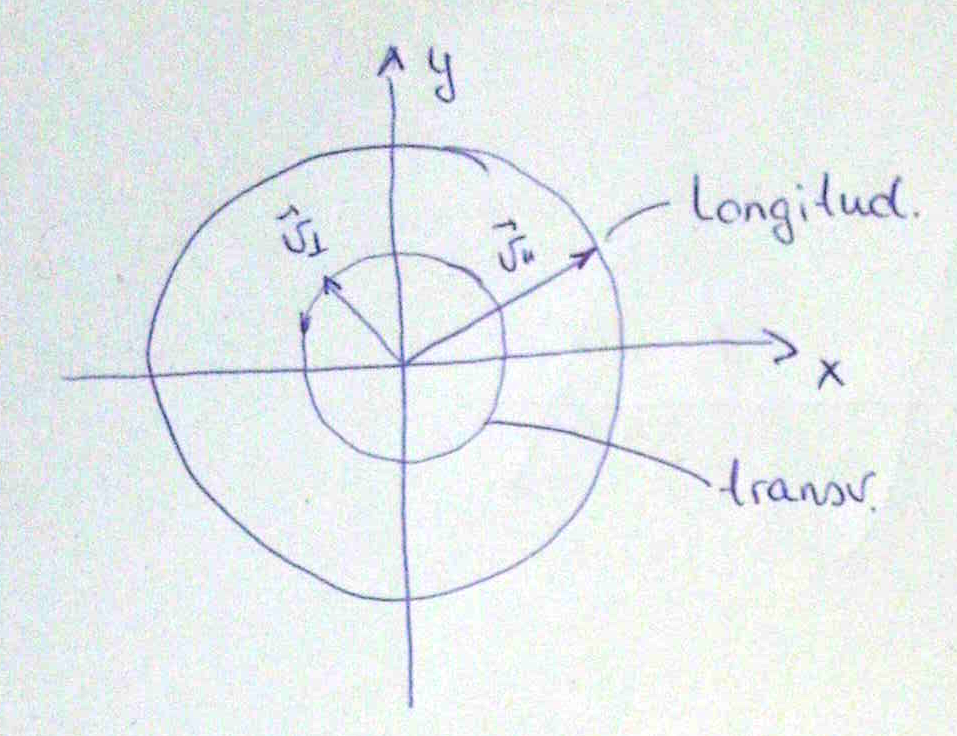
\includegraphics[width=0.75\textwidth]{kap05_02.png}

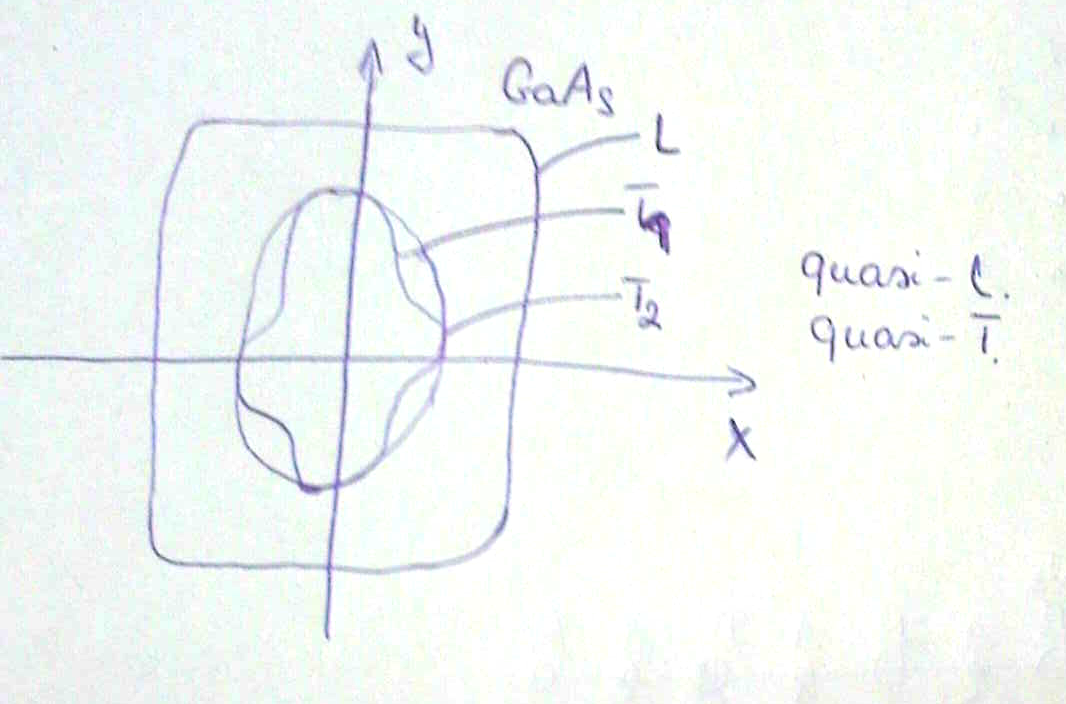
\includegraphics[width=0.75\textwidth]{kap05_03.png}

\end{document}
